
\documentclass{article}
\usepackage[spanish]{babel} %Definir idioma español
\usepackage[utf8]{inputenc} %Codificacion utf-8
\usepackage{amssymb, amsmath, amsbsy, wasysym}
\usepackage{multirow} % para tablas
\usepackage{graphicx}
\title{Tutorial de MATLAB}
\author{Emmanuel Peto Gutiérrez}
\begin{document}
\maketitle

El primer paso es crear una cuenta con el correo de ciencias para tener una licencia en MATLAB. Después, en MATLAB online, se presiona el botón \textit{Learn MATLAB} para ir al tutorial.

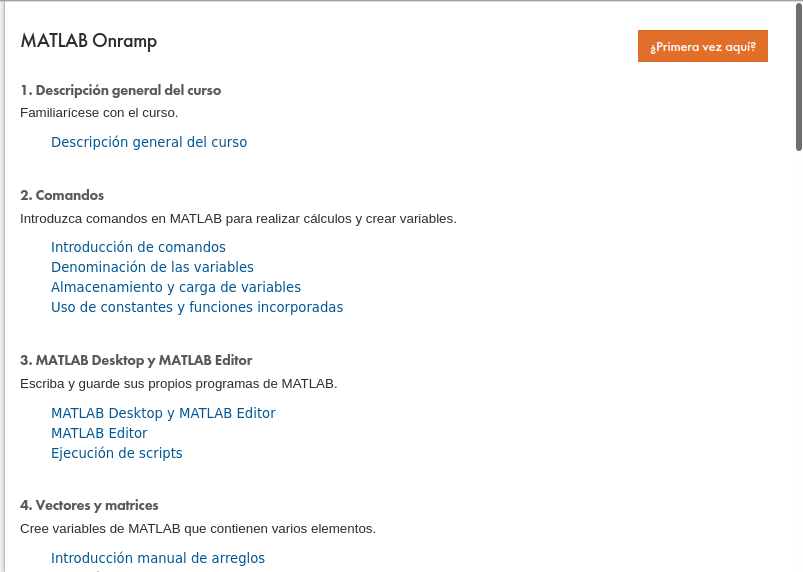
\includegraphics[width=\linewidth]{imagenes/1}

Sección 2: La primera parte es sobre los comandos de MATLAB. Se aprende sobre el uso de variables (como en cualquier lenguaje de programación) y funciones nativas de MATLAB.

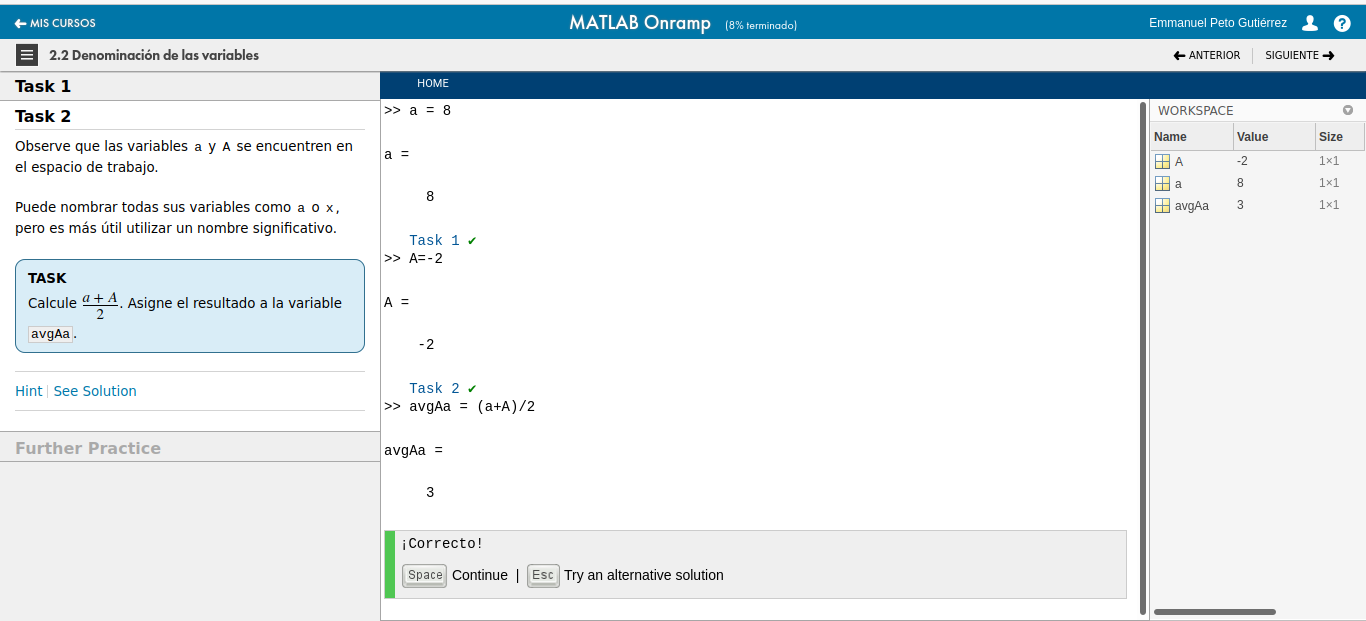
\includegraphics[width=\linewidth]{imagenes/2}

Sección 3: Sobre la edición y ejecución de scripts (o archivos) de MATLAB.

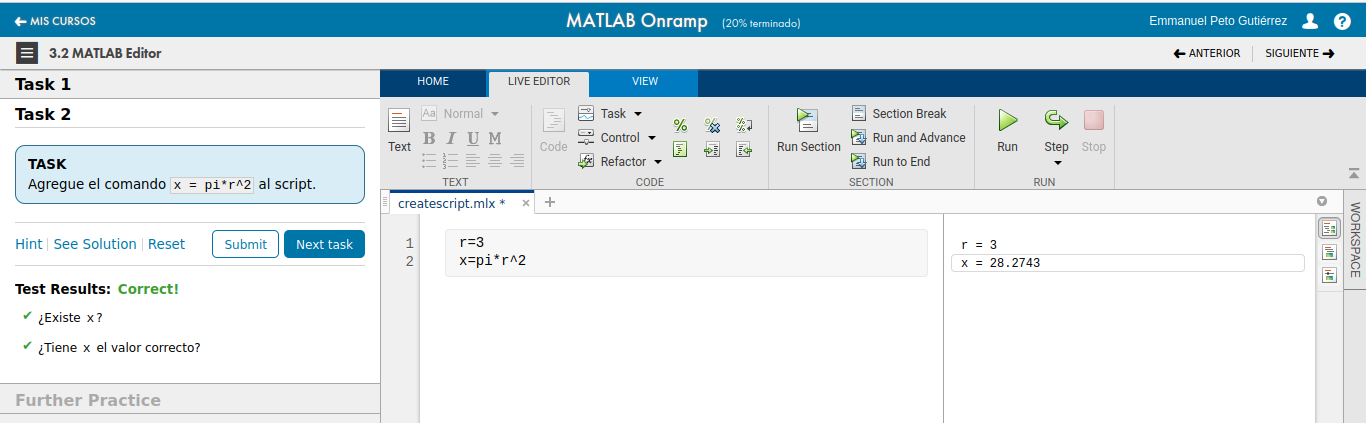
\includegraphics[width=\linewidth]{imagenes/3}

Sección 4: Es sobre la creación de vectores y matrices. En MATLAB cualquier variable se considera un vector de 1x1.

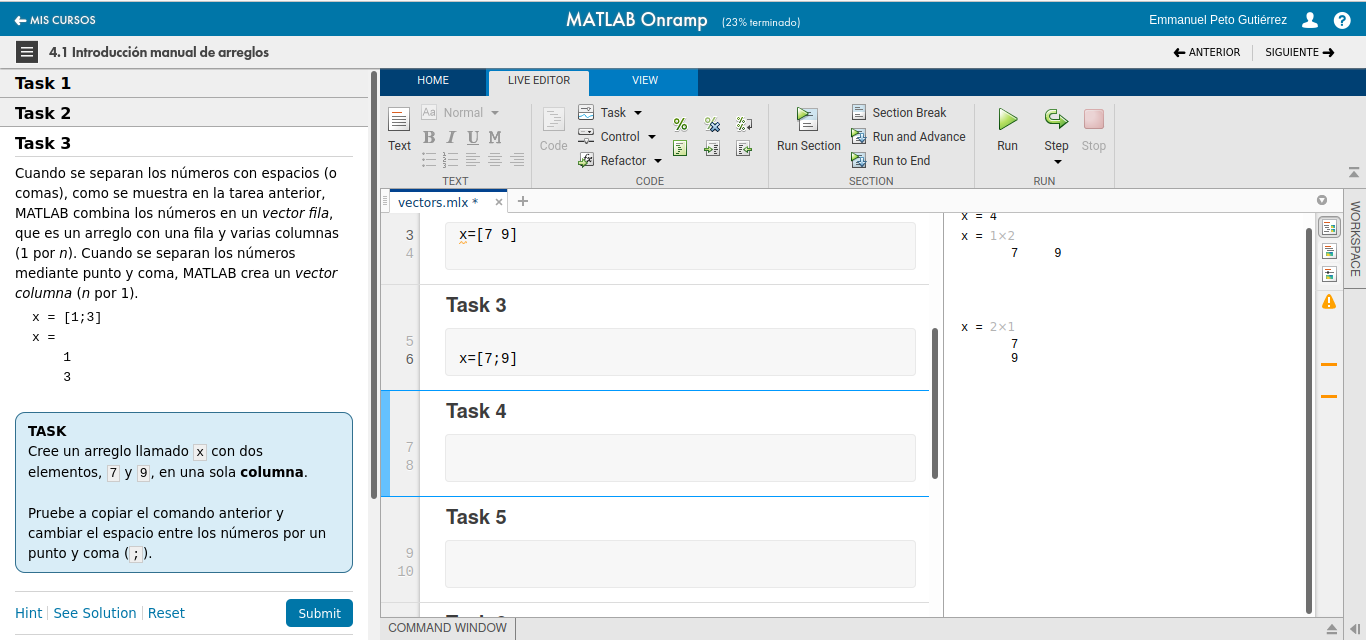
\includegraphics[width=\linewidth]{imagenes/4}

Sección 5: Trata sobre la obtención y modificación de datos en un arreglo o matriz.

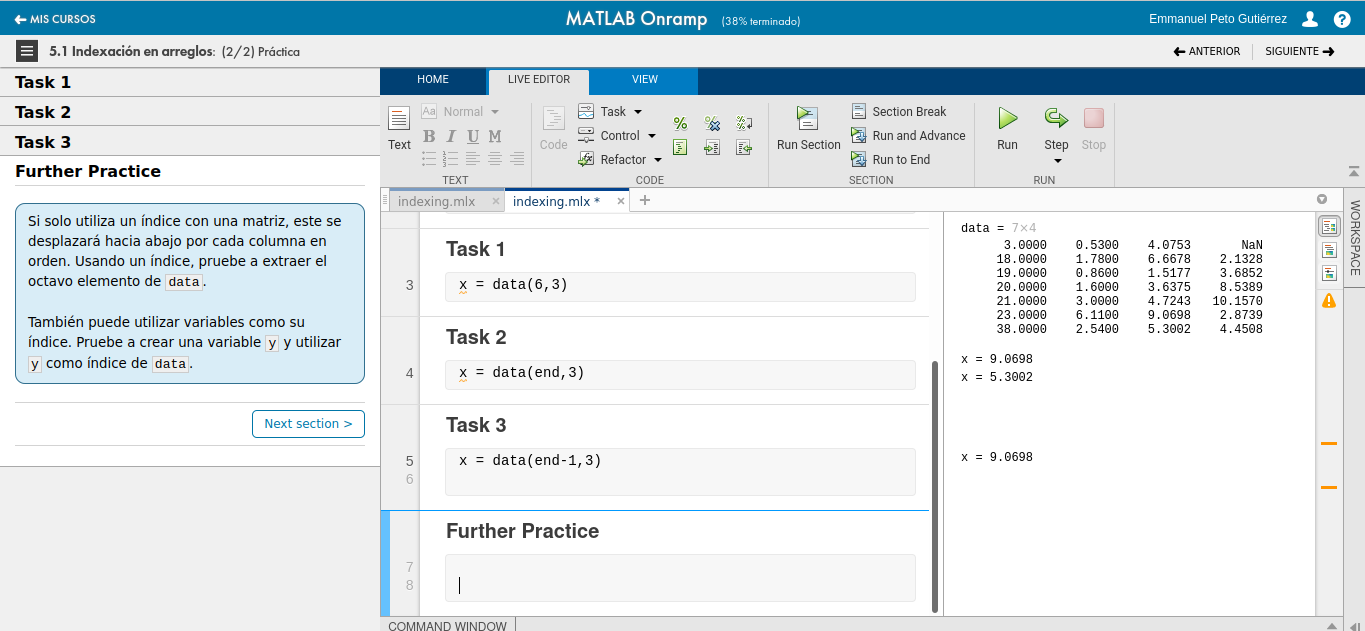
\includegraphics[width=\linewidth]{imagenes/5}

Sección 6: Enseñan cómo realizar operaciones sobre arreglos con un solo comando; por ejemplo, producto punto de dos vectores. Esto es diferente a otros lenguajes donde se tiene que usar un \texttt{for} para recorrer los arreglos.

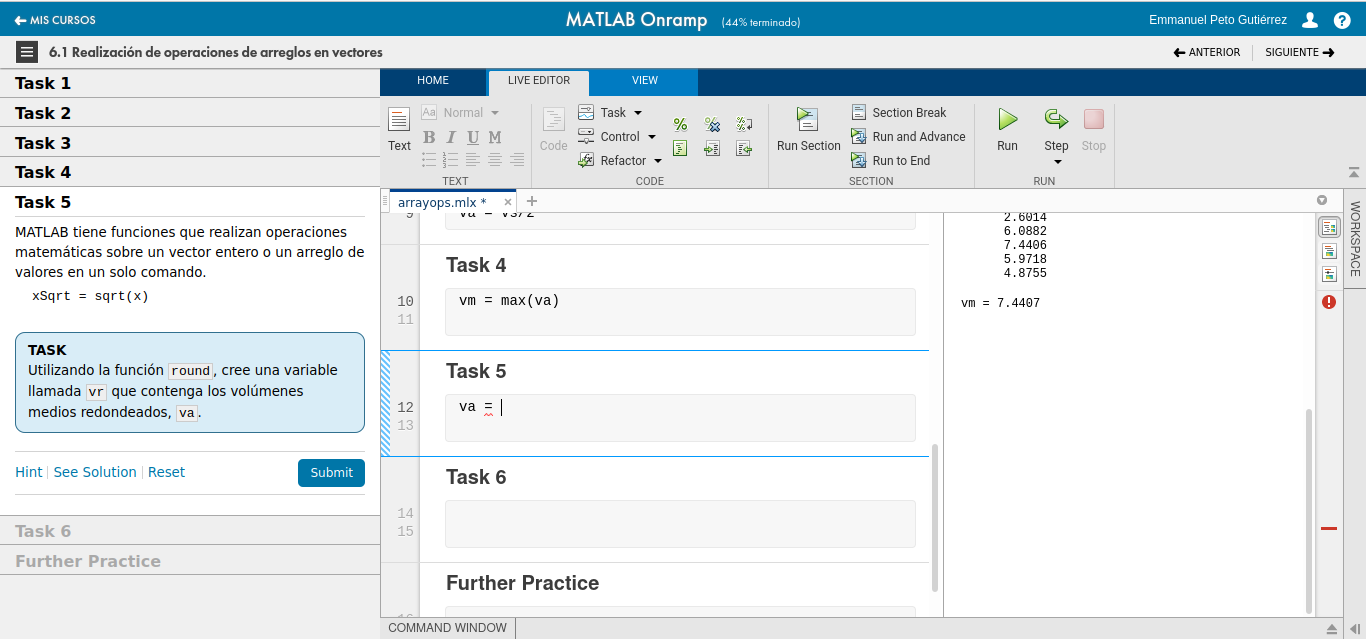
\includegraphics[width=\linewidth]{imagenes/6}

Sección 7: En MATLAB, una misma función puede dar resultados diferentes, dependiendo del parámetro que se le pase y el tipo de variable a la que se le asigna el resultado.

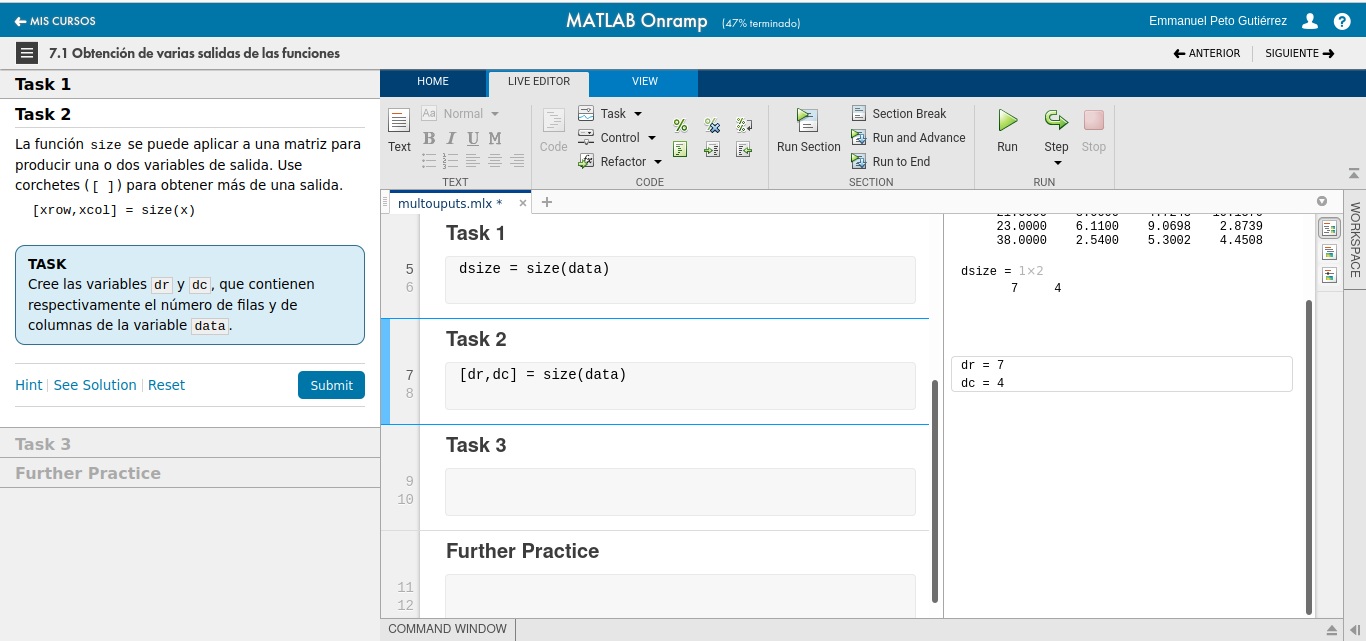
\includegraphics[width=\linewidth]{imagenes/7}

Sección 8: Muestra cómo ver la documentación de MATLAB.

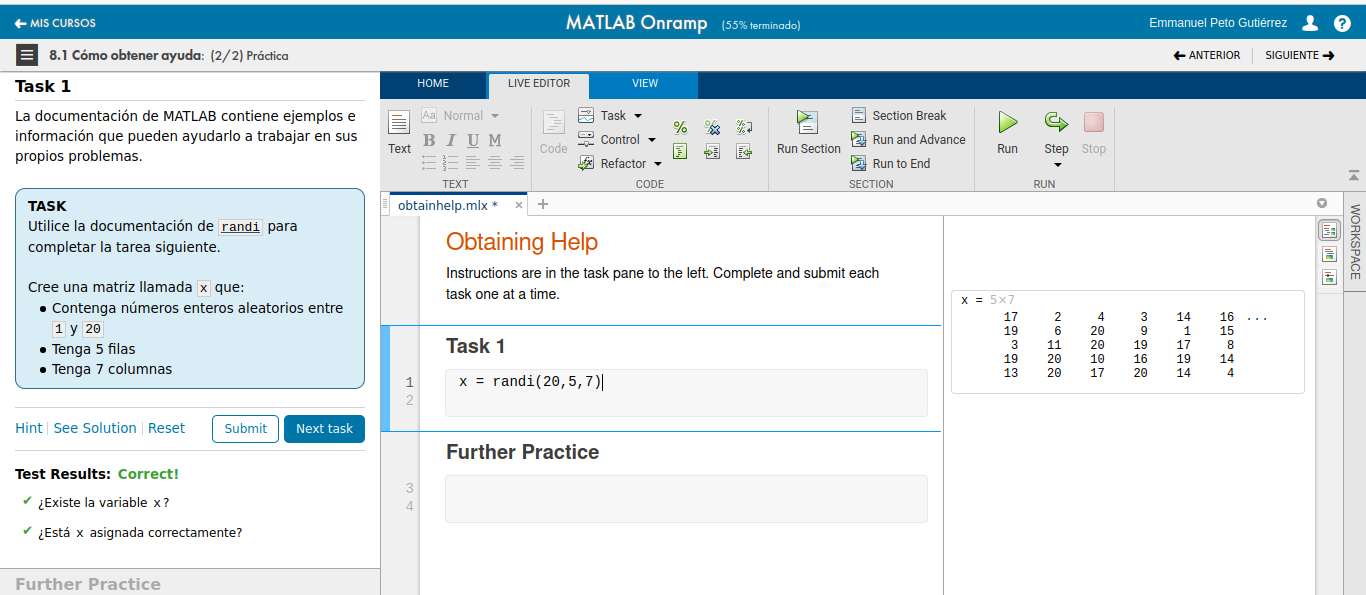
\includegraphics[width=\linewidth]{imagenes/8}

Sección 9: Muestra cómo hacer gráficas de puntos y líneas con los valores en un arreglo o una matriz.

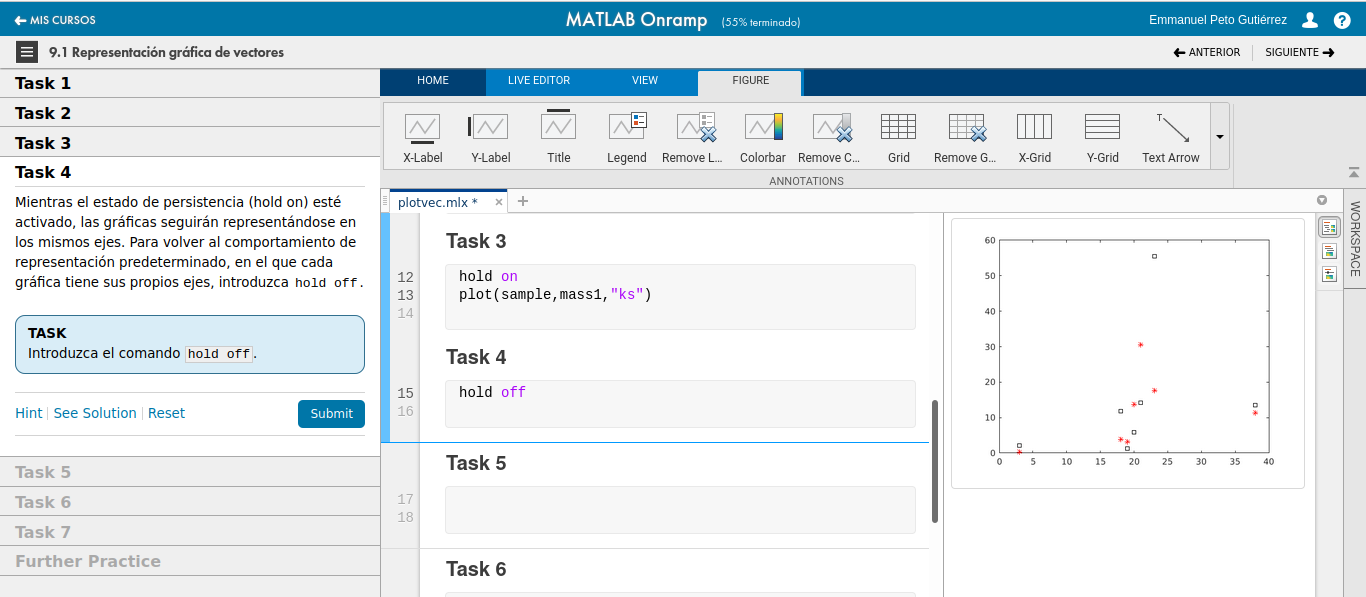
\includegraphics[width=\linewidth]{imagenes/9}

Sección 10: Se realiza un proyecto sobre el consumo de energía eléctrica, usando los conceptos de las secciones anteriores.

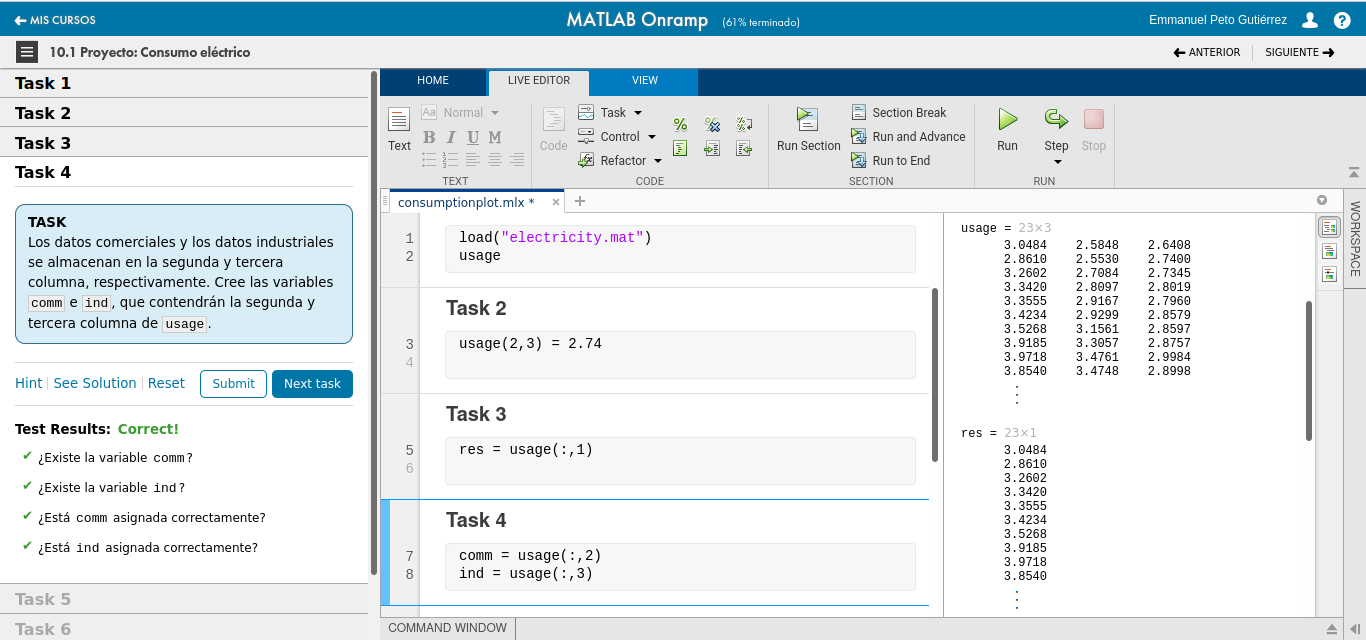
\includegraphics[width=\linewidth]{imagenes/10}

Sección 11: Es sobre la importación de datos hacia un script de MATLAB. Los datos pueden venir de un archivo de texto, una tabla en excel u otro script de MATLAB.

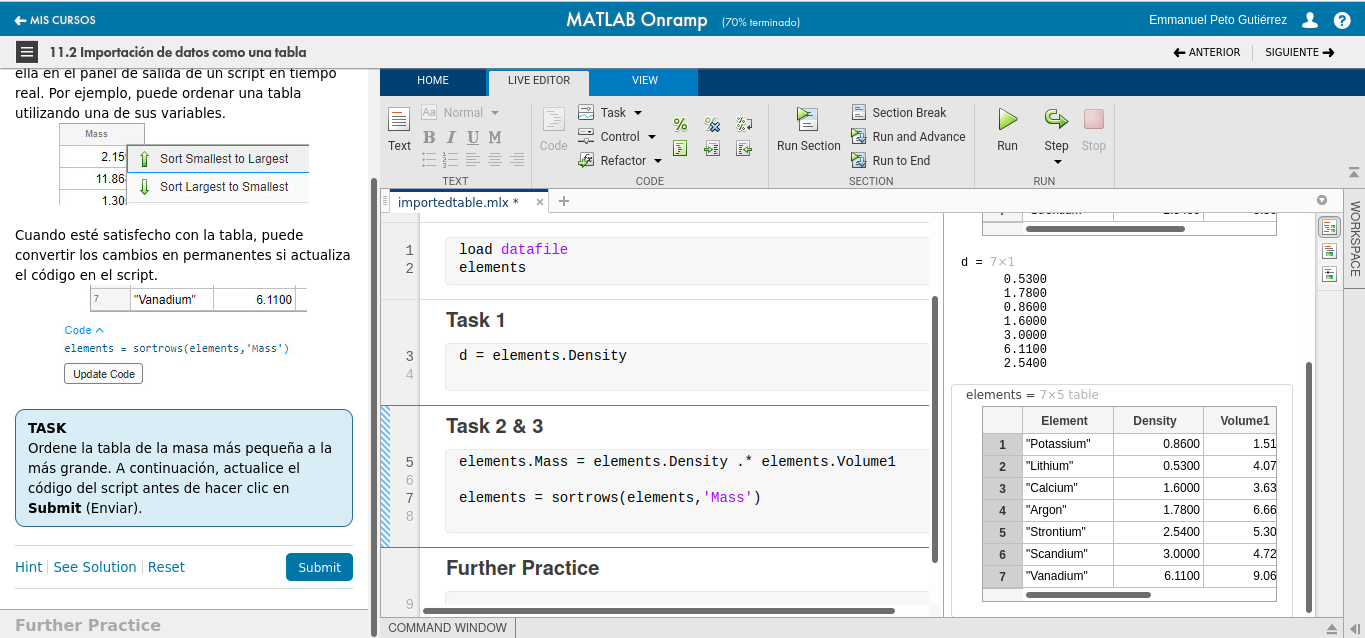
\includegraphics[width=\linewidth]{imagenes/11}

Sección 12: Uso de expresiones lógicas para extraer los datos que cumplan con cierto predicado en un arreglo.

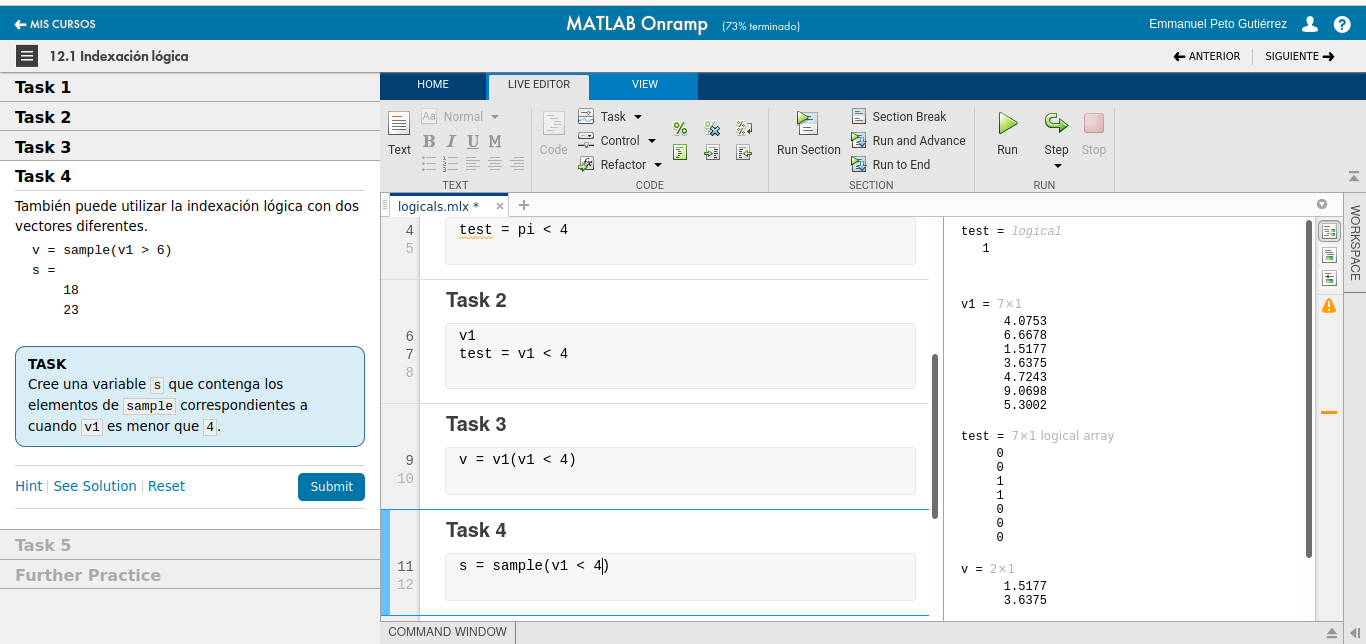
\includegraphics[width=\linewidth]{imagenes/12}

Sección 13: Muestra el uso de ciertas estructuras de control que se usan en otros lenguajes de programación. Las estructuras son: if, else, elseif y for.

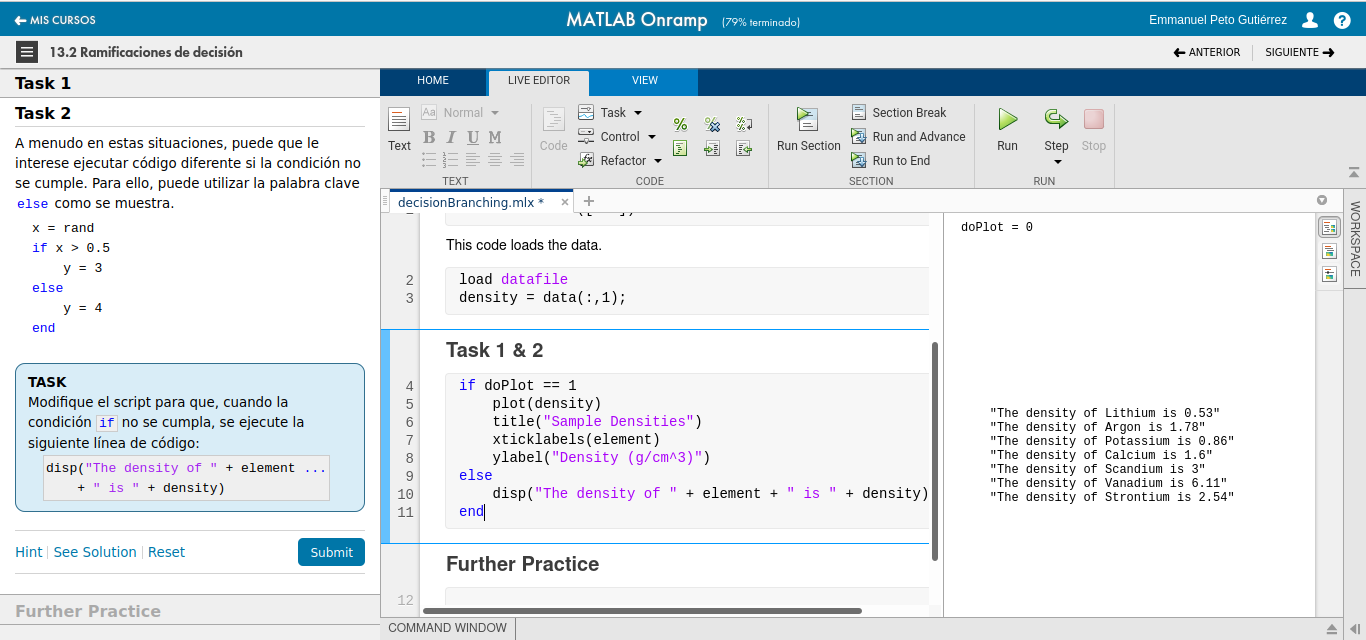
\includegraphics[width=\linewidth]{imagenes/13}

Sección 14: Se realiza un proyecto de ``Movimiento estelar'' usando lo aprendido hasta ahora.

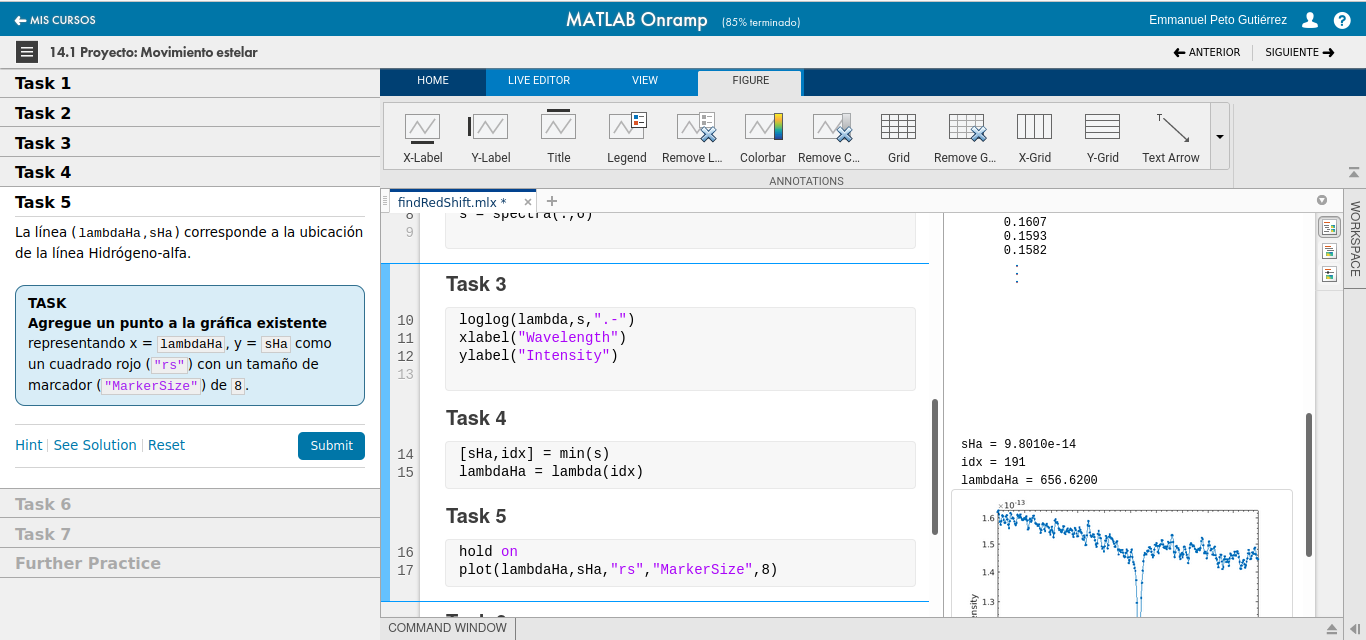
\includegraphics[width=\linewidth]{imagenes/14}

Al final hay que responder una encuesta corta para completar el tutorial al 100\%.

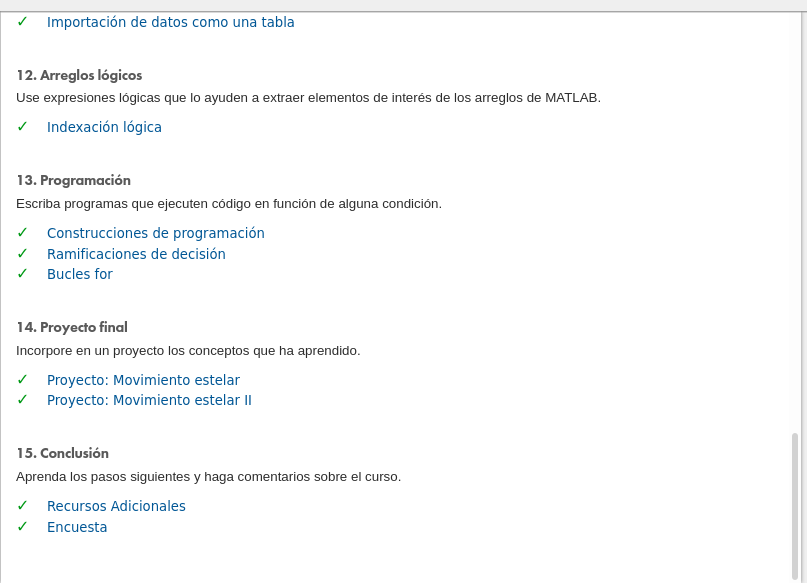
\includegraphics[width=\linewidth]{imagenes/15}

\end{document}

